\chapter{Background}
\label{ch:Background}
In this chapter we recall the required background of the thesis. We start with basic definitions of argumentation frameworks (AFs) in \cref{sec:ArgumentationFrameworks}. Next we treat the clustering of AFs in \cref{sec:ClusteringOfArgumentationFrameworks} and finally we provide a brief overview of SAT-Solvers in \cref{sec:BooleanSatisfiability}.

\section{Argumentation Frameworks}
\label{sec:ArgumentationFrameworks}

Argumentation frameworks were first formally described by Dung in 1995 \cite{DUNG1995321}. They represent an information state, where various conclusions can be drawn from. An AF $G = (A, R)$ consists of two parameters: a set of arguments $A$, and a collection of relations $R$, called attacks which describe the conflicts between the arguments.

They are mostly used in the fields of Artificial Intelligence (AI), e.g.\ in automated reasoning and logic programming \cite{AFINAIARLP, AFINAIARLPexample}. But do also find their applications in other fields like natural language processing \cite{AFINNLP}, trust and reputation systems \cite{AFINTaRS}, legal and medical reasoning \cite{legalAndMedicalReasoning}, and even in game theory and strategic reasoning \cite{AFinGames}.

AFs are represented by directed graph, where the nodes are an abstraction of the arguments $A$, and the arrows represent the attacks $R$. 

\begin{example}
    Let us define an AF $G = (A, R)$ with the arguments
    $A=\{a, b, c, d, e\}$ and the attacks
    $R=\bigl\{(a,b),$
    $(b,b),$
    $(a,c),$
    $(c,a),$
    $(c,d),$
    $(d,e),$
    $(e,d)\bigl\}.$

    This AF can be represented as a directed graph as shown in \cref{af:backgroundAFexample1}.
    \begin{figure}[h]
        \centering
        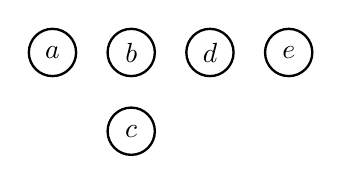
\begin{tikzpicture}
            % Singletons
            \def \ax{0}     \def \ay{0}
            \def \bx{1}     \def \by{0}
            \def \cx{1}     \def \cy{-1}
            \def \dx{2}     \def \dy{0}
            \def \ex{3}     \def \ey{0}

            \draw[line width=0.3mm] (\ax, \ay) circle (0.3) node[anchor=center]{$a$};
            \draw[line width=0.3mm] (\bx, \by) circle (0.3) node[anchor=center]{$b$};
            \draw[line width=0.3mm] (\cx, \cy) circle (0.3) node[anchor=center]{$c$};
            \draw[line width=0.3mm] (\dx, \dy) circle (0.3) node[anchor=center]{$d$};
            \draw[line width=0.3mm] (\ex, \ey) circle (0.3) node[anchor=center]{$e$};

            % Attacks
            \DrawAttackHorizontal{R}{\ax}{\ay}{\bx}{\by}
            \DrawSelfAttackRightSingleton{\bx}{\by}
            \DrawAttackDiagonal{NB}{\ax}{\ay}{\cx}{\cy}
            \DrawAttackDiagonal{PLR}{\cx}{\cy}{\dx}{\dy}
            \DrawAttackHorizontal{B}{\ex}{\ey}{\dx}{\dy}
        \end{tikzpicture}
        \caption{\ac{AF} $G$}
        \label{af:backgroundAFexample1}
    \end{figure}
\end{example}

To be able to conclude something, out of an abstract AF, we need to define semantics. Semantics define subsets of arguments that satisfy semantic-specific rules. Dung already defined different semantics \cite{Dung1995-DUNOTA-2} like conflict-free, admissible and stable.

\newpage
\paragraph{Conflict-Free} According to Dung's definitions, a set is conflict-free if there are no attacks between the arguments in the conflict-free set. A conflict-free set is mainly a building block for the other semantics, which means here that each admissible set or stable extension is conflict-free. We define the set of conflict-free sets of an AF $G$ by $cf(G)$.

\begin{definition}[\cite{Dung1995-DUNOTA-2}]
    Let $G=(A,R)$ be an AF. Then a set $S \subseteq A$ is conflict-free in $G$ if and only if for each $a, b \in S$ we have $(a, b) \not\in R$.
\end{definition}

\begin{example}
    The conflict-free sets of the AF $G$ in \cref{af:backgroundAFexample1} are $\emptyset ,$
    $\{a\},$
    $\{c\},$
    $\{d\},$
    $\{e\},$
    $\{a, d\},$
    $\{a, e\}$ and
    $\{c, e\}$.
\end{example}





\paragraph{Admissible}  A set is admissible, if each attacked argument in the admissible set has a defender in the admissible set.


\begin{definition}[\cite{Dung1995-DUNOTA-2}]
    Let $G=(A,R)$ be an AF. Then a set $S \subseteq A$ is admissible in $G$ if and only if $S \in cf(G)$ and if $a \in S$ with $(b, a) \in R$, then there is a $c \in S$ with $(c, b) \in R$.
\end{definition}
\begin{example}
        The corresponding admissible sets of the AF $G$ in \cref{af:backgroundAFexample1} are $\emptyset ,$
        $\{a\},$
        $\{c\},$
        $\{e\},$
        $\{a, d\},$
        $\{a, e\}$ and
        $\{c, e\}$.
\end{example}



\paragraph{Stable}  An extension is stable if it is conflict-free, and if for every argument, which is not in the stable extension, there exists an attacker in the stable extension.


\begin{definition}[\cite{Dung1995-DUNOTA-2}]
    Let $G=(A,R)$ be an AF. Then a set  $S \subseteq A$ is stable in $G$ if and only if $S \in cf(G), b \not\in S$ implies that there is an $a \in S$ with $(a, b) \in R$.
\end{definition}
\begin{example}
        The stable extensions of the AF $G$ in \cref{af:backgroundAFexample1} are
        $\{a, d\}$ and
        $\{a, e\}$.
\end{example}


The specific rules of a semantics can also be defined via a Boolean formula \cite{inproceedingsBesnardDoutreBooleanFormulaSemantics}. Which then can be used to encode the AFs to be solvable with different solvers like \ac{ASP} \cite{DBLP:journals/corr/abs-1301-1388} or, as in our case, with a \ac{SAT-Solver} \cite{DBLP:journals/amai/AmgoudD13}. Unfortunately, drawing a conclusion from an AF can be challenging, e.g., it can be NP-complete and sometimes even be ''beyond`` NP to decide whether an argument is acceptable (whether there exists, e.g., an admissible set containing ) under a specific argumentation semantics \cite{DBLP:journals/ai/DvorakGRW23}.



\section{Clustering of Argumentation Frameworks}
\label{sec:ClusteringOfArgumentationFrameworks}

When talking about AFs in general, we already have an abstraction layer. By clustering, we add another layer of abstraction where we combine different arguments into one or multiple so called \emph{clusters}. These clustered AFs (i.e.\ abstract AFs) have semantics extensions, just as non-clustered AFs (i.e.\ concrete AFs), which we call abstract semantics extensions. The arguments which are not clustered are called \emph{singletons}. The name is derived from set theory, where singleton refers to a set containing exactly one argument.
By definition, a cluster is a single entity (composed of multiple arguments) which can be integrated in an AF to reduce the complexity. While reducing the overall complexity of the AF with clusters, we add a new computation layer: computing \emph{faithful} clustered AFs. The term \emph{faithful} describes the property of a clustered AF, that every abstract semantics extension can be mapped to a concrete semantics extension. If the clustered AF creates a semantics set which cannot be mapped to a concrete set, we call it \emph{spurious}.

Clustered abstract AFs can also be modelled with graphs. One can represent each singleton argument as a node, attacks as arrows, and each cluster can be represented by a rectangle with every clustered argument inside of it. Let us have a look at an example and define AF $\hat{G}=(\hat{A}, \hat{R})$ with the arguments $\hat{A}=\{d, e, \hat{h}\}$, where the cluster $\hat{h}$ contains the arguments $\{a, b, c, d\}$ and the attacks being $\hat{R}=\bigl\{(\hat{h}, d)$, $(d, e)$, $(e, d)$, $(\hat{h},\hat{h})\bigl\}$.  This AF can be represented as a directed graph as shown in \cref{af:backgroundExampleClusterSpurious}.


\begin{figure}[h]
    \centering
    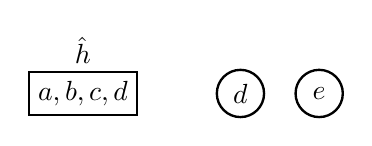
\begin{tikzpicture}
        % Singletons
        \def \ex{3}     \def \ey{0}
        \def \dx{2}     \def \dy{0}
        \def \hx{0}     \def \hy{0}

        \node[rectangle, draw, line width=0.3mm] at (\hx, \hy) {$a,b,c,d$};
        \node at (0, 0.55) {$\hat{h}$};
        \draw[line width=0.3mm] (\ex, \ey) circle (0.3) node[anchor=center]{$e$};
        \draw[line width=0.3mm] (\dx, \dy) circle (0.3) node[anchor=center]{$d$};

        % Attacks
        \DrawSelfAttackLeftTopCluster{\hx-0.65}{\hy + 0.3}
        \DrawAttackHorizontal{R}{\hx+0.5}{\hy}{\dx}{\dy}
        \DrawAttackHorizontal{B}{\ex}{\ey}{\dx}{\dy}
    \end{tikzpicture}
    \caption{\ac{AF} $\hat{G}$ clustered}
    \label{af:backgroundExampleClusterSpurious}
\end{figure}


%\textit{TODO: Definition of Semantics}
Since clusters can not be treated the exact same way as an argument, we need to refine the definitions of the semantics. When referring to the alternative semantics used in clustered AFs, we call them \emph{abstract} semantics (e.g.\ abstractly conflict-free ($\hat{cf}$), abstractly admissible ($\hat{adm}$) and abstractly stable ($\hat{stb}$)). Let us consider a clustered AF $\hat{G}=\{\hat{A}, \hat{R}\}$ and redefine the semantics.

\paragraph{Conflict-Free} A set of arguments is abstractly conflict-free, if there is no attack between the singletons of the set.

\begin{definition}[\cite{DBLP:conf/kr/SaribaturW21}]
    Let $\hat{G}=(\hat{A},\hat{R})$ be an AF. Then a set  $S \subseteq \hat{A}$ is conflict-free in $\hat{G}$ if and only if for each $\hat{a}, \hat{b} \in$ singleton($S$) we have $(\hat{a}, \hat{b}) \not\in \hat{R}$.
\end{definition}

\begin{example}
    The abstractly conflict-free sets of the abstract AF $G$ in \cref{af:backgroundExampleClusterSpurious} are 
    $\{\},$
    $\{d\}$,
    $\{e\}$,
    $\{\hat{h}\}$,
    $\{e, \hat{h}\}$,
    $\{d, \hat{h}\}$.
\end{example}




\paragraph{Admissible} A set of arguments is abstractly admissible, if it is abstractly conflict-free and if every singleton which is being attacked, has a defender.

\begin{definition}[\cite{DBLP:conf/kr/SaribaturW21}]
    Let $\hat{G}=(\hat{A},\hat{R})$ be an AF. Then a set  $S \subseteq \hat{A}$ is admissible in $\hat{G}$ if and only if $S \in \hat{cf}(\hat{G})$ and if $\hat{a} \in S$ with $(\hat{b}, \hat{a}) \in \hat{R}$ with singleton($\hat{a}$), then there is a $\hat{c} \in \hat{G}$ with $(\hat{c}, \hat{b}) \in \hat{R}$.
\end{definition}
\begin{example}
    The abstractly admissible sets of the abstract AF $G$ in \cref{af:backgroundExampleClusterSpurious} are $\{\},$
    $\{e\}$,
    $\{\hat{h}\}$,
    $\{e, \hat{h}\}$,
    $\{d, \hat{h}\}$.
\end{example}





\paragraph{Stable} A set of arguments is abstractly stable, if it is abstractly conflict-free and if an argument is not in the abstractly stable extension, it implies that an argument in the abstractly stable extension is attacking it. Furthermore if the abstractly stable extension is not attacking an argument, then every singleton attacking the argument is not in the abstractly stable extension.

\begin{definition}[\cite{DBLP:conf/kr/SaribaturW21}]
    Let $\hat{G}=(\hat{A},\hat{R})$ be an AF. Then an extension $S \subseteq \hat{A}$ is stable in $\hat{G}$ if and only if $S \in \hat{cf}(\hat{G}), \hat{b} \not\in S$ implies that there is an $\hat{a} \in \hat{S}$ with $(\hat{a}, \hat{b}) \in \hat{R}$, and if $S$ does not attack an $\hat{a} \in S$ then $\hat{b} \not\in S$ whenever $(\hat{a}, \hat{b}) \in \hat{R}$ and singleton $(\hat{b})$.
\end{definition}


\begin{example}
    The abstractly stable extensions of the abstract AF $G$ in \cref{af:backgroundExampleClusterSpurious} are
    $\{e, \hat{h}\}$,
$\{d, \hat{h}\}$.
\end{example}


Let us have a look at a concrete example to explain faithfulness. The concrete AF $G=(A, R)$ has the following arguments $A=\{a, b, c, d, e\}$ with these attacks:
$R=\bigl\{(a,b),$
$(b,b),$
$(a,c),$
$(c,a),$
$(c,d),$
$(d,e),$
$(e,d)\bigl\}$. This AF can be represented as a directed graph shown in \cref{fig:BackgroundClusteringOfArgumentsExampleDouble}(a).

Now we can group the arguments $\{a, b, c, d\}$ together into one single cluster $\hat{h}$. The arguments for the abstract AF $\hat{G}=(\hat{A}, \hat{R})$ would then be $\hat{A}=\{e, \hat{h}\}$, where the cluster $\hat{h}$ is composed of $\{a, b, c, d\}$ and the according attacks are
$\hat{R}=\bigl\{(\hat{h}, e), (e, \hat{h}), (\hat{h}, \hat{h})\bigl\}$. The attacks are directly derived from the concrete AF. If an argument is clustered, the cluster inherits the attacks from the argument. The emerging AF can be represented as a directed graph shown in \cref{fig:BackgroundClusteringOfArgumentsExampleDouble}(b).


\vspace{0.3cm}
\begin{figure}[h]
    \centering
    \begin{subfigure}[t]{0.45\textwidth}
        \centering
        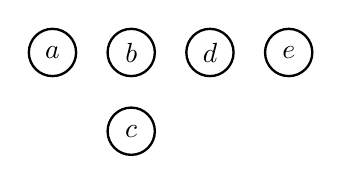
\begin{tikzpicture}
            % Singletons
            \def \ax{0}     \def \ay{0}
            \def \bx{1}     \def \by{0}
            \def \cx{1}     \def \cy{-1}
            \def \dx{2}     \def \dy{0}
            \def \ex{3}     \def \ey{0}
    
            \draw[line width=0.3mm] (\ax, \ay) circle (0.3) node[anchor=center]{$a$};
            \draw[line width=0.3mm] (\bx, \by) circle (0.3) node[anchor=center]{$b$};
            \draw[line width=0.3mm] (\cx, \cy) circle (0.3) node[anchor=center]{$c$};
            \draw[line width=0.3mm] (\dx, \dy) circle (0.3) node[anchor=center]{$d$};
            \draw[line width=0.3mm] (\ex, \ey) circle (0.3) node[anchor=center]{$e$};
    
            % Attacks
            \DrawAttackHorizontal{R}{\ax}{\ay}{\bx}{\by}
            \DrawSelfAttackRightSingleton{\bx}{\by}
            \DrawAttackDiagonal{NB}{\ax}{\ay}{\cx}{\cy}
            \DrawAttackDiagonal{PLR}{\cx}{\cy}{\dx}{\dy}
            \DrawAttackHorizontal{B}{\ex}{\ey}{\dx}{\dy}
        \end{tikzpicture}
        \subcaption{Concrete AF $G$}
        \label{af:backgroundClusterExample1}
    \end{subfigure}%
    \begin{subfigure}[t]{0.45\textwidth}
        \centering
        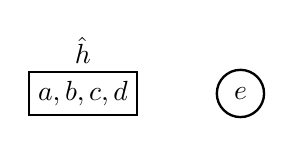
\begin{tikzpicture}
            % Singletons
            \def \ex{2}     \def \ey{0}
            \def \hx{0}     \def \hy{0}
    
            \node[rectangle, draw, line width=0.3mm] at (\hx, \hy) {$a,b,c,d$};
            \node at (0, 0.55) {$\hat{h}$};
            \draw[line width=0.3mm] (\ex, \ey) circle (0.3) node[anchor=center]{$e$};
    
            % Attacks
            \DrawSelfAttackLeftTopCluster{\hx-0.65}{\hy + 0.3}
            \DrawAttackHorizontal{B}{\ex}{\ey}{\hx+0.5}{\hy}
        \end{tikzpicture}
        \subcaption{Abstract AF $\hat{G}$}
        \label{af:backgroundClusterExample2}
    \end{subfigure}
    \caption{Concrete and abstract AF}
    \label{fig:BackgroundClusteringOfArgumentsExampleDouble}
\end{figure}



If we compare the stable extensions of the concrete AF $G$ (e.g.\ 
$stb(G)=\bigl\{\{a, e\}$, $\{a, d\}$ $\bigl\}$) with the abstractly stable extensions of the abstract clustered AF $\hat{G}$ (e.g.\ 
$\hat{stb}(G)=\bigl\{$ 
$\{\hat{h}\}$, 
$\{e\}$, 
$\{e, \hat{h}\}$ 
$\bigl\}$), 
we see that it is spurious due to the abstractly stable extension $\{e\}$ which cannot be mapped to one of the concrete stable extensions. The mapping of semantics extensions with clustered AFs is done the same way as for concrete AFs, except that clusters can mutate to every possible combination of the clustered Arguments. In our example, the cluster $\hat{h}$ can mutate to
$\{a\}$, 
$\{b\}$, 
$\{c\}$, 
$\{d\}$, 
$\{a, b\}$, 
$\{a, c\}$, 
$\{a, d\}$, 
$\{b, c\}$, 
$\{b, d\}$, 
$\{c, d\}$, 
$\{a, b, c\}$, 
$\{a, b, d\}$, 
$\{a, c, d\}$, 
$\{b, c, d\}$ and
$\{a, b, c, d\}$.
To create a faithful clustered AF, we can concretize one or more arguments of the cluster. By concretizing the argument $\{d\}$, we obtain a new AF $\hat{G}'=(\hat{A}', \hat{R}')$ with the arguments $\hat{A}'=\{d, e, \hat{h}\}$, where the cluster $\hat{h}$ is composed of $\{a, b, c\}$, and the corresponding attacks are $\hat{R}'=\{(d, \hat{h}),$
$(d, e),$
$(e, d),$
$(\hat{h}, \hat{h})\}$.

With this definition we can build the concretized abstract graph $\hat{G}'$ in \cref{af:backgroundClusterExample3}.


\begin{figure}[h]
    \centering
    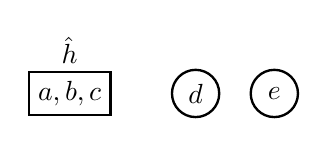
\begin{tikzpicture}
        % Singletons
        \def \ex{3}     \def \ey{0}
        \def \dx{2}     \def \dy{0}
        \def \hx{0.4}     \def \hy{0}

        \node[rectangle, draw, line width=0.3mm] at (\hx, \hy) {$a,b,c$};
        \node at (0.4, 0.55) {$\hat{h}$};
        \draw[line width=0.3mm] (\ex, \ey) circle (0.3) node[anchor=center]{$e$};
        \draw[line width=0.3mm] (\dx, \dy) circle (0.3) node[anchor=center]{$d$};

        % Attacks
        \DrawSelfAttackLeftTopCluster{\hx-0.42}{\hy + 0.3}
        \DrawAttackHorizontal{R}{\hx+0.25}{\hy}{\dx}{\dy}
        \DrawAttackHorizontal{B}{\ex}{\ey}{\dx}{\dy}
    \end{tikzpicture}
    \caption{Concretized AF $\hat{G}'$}
    \label{af:backgroundClusterExample3}
\end{figure}

Every abstractly stable extension in \cref{af:backgroundClusterExample3} (e.g.\ $\{d, \hat{h}\}, \{e, \hat{h}\})$ can be mapped to one of the concrete stable extensions of $G$, which means that the clustered AF $\hat{G}'$ is faithful.


\section{Boolean Satisfiability}
\label{sec:BooleanSatisfiability}

A SAT(isfability)-Solver is used to compute Boolean formulas in an efficient way \cite{Biere2009}. The main purpose is to determine if a formula is satisfiable (e.g.\ the variables of the formula can be set to \emph{true} or \emph{false} s.t.\ the expression evaluates to \emph{true}). If no combination of setting the variables to \emph{true} or \emph{false} s.t.\ the formula evaluates to \emph{true} is found, we call the Boolean expression UNSAT(isfiable). Most of the SAT-Solvers do also provide a model, if a Boolean expression is satisfiable. A model in this context is an assignment of truth values to the variables that satisfies a given Boolean formula. The Boolean formula is composed of different logical operators, i.e.\ negation ($\lnot$), conjunction ($\land$), disjunction ($\lor$) and implication ($\rightarrow$). The corresponding truth tables are defined in \cref{table:BackgroundLogicalOperators}.

\begin{figure}[h!]
    \captionof{table}{Boolean logic operators}
    \label{table:BackgroundLogicalOperators}
    \centering
    \begin{minipage}{.18\textwidth}
        \centering
        \subcaption{Negation}
        \begin{tabular}{|c|c|}
        \hline
        x & $\lnot$ \\
        \hline
        0 & 1\\
        \hline
        1 & 0\\
        \hline
        \end{tabular}
        \vspace{0.96cm}
    \end{minipage}%
    \begin{minipage}{.18\textwidth}
        \centering
        \subcaption{Conjunction}
        \begin{tabular}{|c|c|c|}
            \hline
            x & y & $\land$ \\
            \hline
            0 & 0 & 0\\
            \hline
            0 & 1 & 0\\
            \hline
            1 & 0 & 0\\
            \hline
            1 & 1 & 1\\
            \hline
            \end{tabular}
    \end{minipage}
    \begin{minipage}{.18\textwidth}
        \centering
        \subcaption{Disjunction}
        \begin{tabular}{|c|c|c|}
            \hline
            x & y & $\lor$ \\
            \hline
            0 & 0 & 0\\
            \hline
            0 & 1 & 1\\
            \hline
            1 & 0 & 1\\
            \hline
            1 & 1 & 1\\
            \hline
            \end{tabular}
    \end{minipage}
    \begin{minipage}{.18\textwidth}
        \centering
        \subcaption{Implication}
        \begin{tabular}{|c|c|c|}
            \hline
            x & y & $\rightarrow$ \\
            \hline
            0 & 0 & 1\\
            \hline
            0 & 1 & 1\\
            \hline
            1 & 0 & 0\\
            \hline
            1 & 1 & 1\\
            \hline
            \end{tabular}
    \end{minipage}
\end{figure}



SAT-Solvers do find there applications in various domains, e.g.\ in verification and validation of software and hardware \cite{DBLP:conf/dagstuhl/Gogolla09, DBLP:books/daglib/0045943}. But also in AI and machine learning \cite{DBLP:phd/basesearch/Liang18a} and even in security~\cite{Pasero2022-SATHashFunctions-Repo, DBLP:journals/iacr/LinYXTS24}.

The decision problem of deciding whether a Boolean formula is satisfiable (SAT) is NP-complete, and it was the first problem to be shown to be NP-complete \cite{Cook71}. Subsequently, many other problems were shown to be NP-hard, due to a reduction from SAT.

Each year further optimizations of SAT-solvers are developed. There are several competitions which are being ran in different classes \cite{SAT-Solver-Competition}. Meanwhile, SAT-Solvers are so specialized, that there is no overall best SAT-Solver, but it is dependent on the application field. An overall good performing and easy to implement SAT-Solver, which we also used in this thesis is the z3 SAT-Solver \cite{z3-SAT-Solver}.







